\begin{document}

% Front matter
\frontmatter

%% r.1 blank page
%\blankpage
%
%% v.2 epigraphs
%\newpage\thispagestyle{empty}
%\openepigraph{%
%The public is more familiar with bad design than good design.
%It is, in effect, conditioned to prefer bad design, 
%because that is what it lives with. 
%The new becomes threatening, the old reassuring.
%}{Paul Rand%, {\itshape Design, Form, and Chaos}
%}
%\vfill
%\openepigraph{%
%A designer knows that he has achieved perfection 
%not when there is nothing left to add, 
%but when there is nothing left to take away.
%}{Antoine de Saint-Exup\'{e}ry}
%\vfill
%\openepigraph{%
%\ldots the designer of a new system must not only be the implementor and the first 
%large-scale user; the designer should also write the first user manual\ldots 
%If I had not participated fully in all these activities, 
%literally hundreds of improvements would never have been made, 
%because I would never have thought of them or perceived 
%why they were important.
%}{Donald E. Knuth}


% r.3 full title page
\maketitle


% v.4 copyright page
\newpage
\begin{fullwidth}
	{\large {\it Author\ \ } Vic Smith, Laith Alissa, Jon Cave, Joey Squidballs
	
	\vspace{1em}\noindent{\it Supervisor\ \ } Sara Kalvala
	
	\vspace{1em}\noindent{\it Abstract\ \ } Bla, bla, bla, abstract...
	
	\vspace{1em}\noindent{\it Keywords\ \ } Functional Programming, Haskell, Games, etc
	
	}
	
	~\vfill
	\thispagestyle{empty}
	\setlength{\parindent}{0pt}
	\setlength{\parskip}{\baselineskip}
	Copyright \copyright\ \the\year\ \thanklessauthor
	
	\par\smallcaps{Published by \newlinetospace{\thanklesspublisher}}
	
	%\par\smallcaps{Typesetting: tufte-latex.googlecode.com}
	
	\par Licensed under the Apache License, Version 2.0 (the ``License''); you may not
	use this file except in compliance with the License. You may obtain a copy
	of the License at \url{http://www.apache.org/licenses/LICENSE-2.0}. Unless
	required by applicable law or agreed to in writing, software distributed
	under the License is distributed on an \smallcaps{``AS IS'' BASIS, WITHOUT
	WARRANTIES OR CONDITIONS OF ANY KIND}, either express or implied. See the
	License for the specific language governing permissions and limitations
	under the License.\index{license}
	
	\par\textit{First printing, \monthyear}


% r.5 contents
\tableofcontents

\end{fullwidth}
%\listoffigures

%\listoftables

%\lstlistoflistings

 %r.7 dedication
\cleardoublepage
~\vfill
\begin{doublespace}
\noindent\fontsize{18}{22}\selectfont\itshape
\nohyphenation
Dedicated to...
\end{doublespace}
\vfill
\vfill


%%
% Start the main matter (normal chapters)
\mainmatter

% r.9 introduction
\chapter[Foreword]{Foreword}
\label{ch:forward}

\chapterepigraph{``Perhaps it hasn't one," Alice ventured to remark. ``Tut, tut, child!" said the Duchess. ``Everything's got a moral, if only you can find it."}{from Lewis Carol's  \emph{Alice in Wonderland}}

\newthought{Starting a sentance} with a newthought.

\section{A Section}

Lorum ipsum dolor sit amet.
\input{chapter/frontmatter/brief}

\part{Project Initiation and Planning\label{part:pid}}
	\chapter[Motivation]{Motivation}
\label{ch:motivation}

\chapterepigraph{If you aren't sure which way to do something, then do it both ways and see which works better.}{John Carmack}

\newthought{Functional programming} has a long history, with its roots in the $\lambda$-calculus of Alonzo Church.\citefix[-1.5em]{church1932} One of the first functional programming languages was Lisp, invented by John McCarthy in the 1958; and Lisp is still used today, over 50 years later.\citepage{reilly2003}{pages 156--157} Various languages have refined and extended the paradigm over the years --- probably the most notable as of now being Haskell, Scala, OCaml, F\#, and Erlang.

Despite the amount of time such languages have been available, use in industry has typically been far less than that of languages such as C, C++, and Java.\citepage[-2em]{odersky2010programming}{page 11} That being said, in recent years there has been increasing use of functional techniques and languages in certain areas. Erlang was designed for the development of highly fault tolerant telecommunication systems.\cite[-1em]{armstrong2007history} OCaml is used in the financial sector to create trading algorithms.\citefix[1em]{minsky2011ocaml} Scala is increasingly popular, helped 

One of the often cited reasons against the use of functional programming in some domains is that of performance. This is due in part to mutable data structures generally being easier to represent on machine hardware; and it therefore being harder for functional compilers to convert the code into an efficient representation.\citefix{paulson1996ml} However, it is not a given that any program would run slower if written in a functional language: in some cases lazy-evaluation or compiler optimisations made possible by immutability can mean a program runs faster, plus advanced compiler techniques such as array fusion can lead to programs nearing the efficiency of hand-crafted C. And with modern machines getting ever faster, the domain of problems that require high levels of efficiency is getting smaller.

Performance problems alone cannot account for the fringe position of functional programming. The efficacy and advantages of the functional approach to programming and problem solving have been stated many times over a considerable number of years,\citefix{hughes1989functional} yet it is still rare for mainstream projects to make any use of functional languages or tools.

Instead of researching and discussing the theoretical advantages of the functional paradigm, this project instead will attempt to demonstrate the value of functional programming by utilising it in a problem domain that should pose a significant  challenge, that is not normally considered a `good' domain for FP. 

\section{Why a Game?}

Game programming brings together a diverse range of computing areas. A game involves human interaction in real time, detailed graphics and animation, artificial intelligence / planning, networking, and various other dynamic elements. A game is also 

\section{Why Haskell?}
	\chapter[Project Requirements]{Project Requirements}
\label{ch:reference}

\chapterepigraph{Rien n'est plus difficile, et donc plus pr\'ecieux, que d'\^etre capable de d\'ecider}{Napol\'eon Bonaparte}

\newthought{Here presented are the aims}, endpoints, controls, methods, schedule, and every relevant detail of the project; laid out unequivocally for reference before, during, and after the required work.

\section{Objectives and Deliverables}

\begin{margintable}
\vspace{12em}
\renewcommand{\arraystretch}{1.5}
\begin{tabular}
{p{8em} p{7em}}
		\toprule
		\emph{Deliverable} & \emph{Deadline} \\
		\midrule
		Prototype Game & Dec 6th 2012\\
		Progress Poster & Dec 6th 2012\\
		Final game & April 25th 2013\\
		Report & April 25th 2013\\
		Presentation & May 7th 2013 \\
		\bottomrule
\end{tabular}
\vspace{0.5em}
\caption{Summary of Deadlines}
\end{margintable}

The first objective of the project team is to produce a playable prototype of the game specified. 
The prototype can be extremely basic, provided the playing experience gives a promising outlook for the final release. The prototype release is both an internal motivating factor and a requirement for the progress report at the end of term 1.

The progress poster is the first external deadline, and is a customer requirement for ensuring the project is on schedule. The progress poster will contain technical detail of the project progress to date, as well as screen captures of the latest running game prototype.

The final game should be completed to the requirements laid out in the specification and to amendments agreed on by the customer. An end user should be able to play a networked game with minimal configuration (no more configuration required than a typical installation and networking configuration).

The presentation and final report are the last deliverables of the project. They give the team the opportunity to deconstruct the project's progress over the academic year, and give an analysis of the finished product. The report documents the design approach taken, relevant research which influenced the project, quality standards review, testing, user manuals, and any critical decisions made during the project, and the presentation will give the project team a chance to introduce the game, and offers the customer an opportunity to question the team. 

%might need to rephrase the double and

\chapter[Requirements]{Requirements}
\label{ch:requirements}

\chapterepigraph{``All things are created twice; first mentally; then physically.  The key to creativity is to begin with the end in mind, with a vision and a blue print of the desired result."}{ Stephen Covey}

\newthought{Starting a sentence} with a new thought.


% help site at http://www.projectmanagementhelp.com/how-to-write-functional-requirements/
% bullet point these requirements, describe them, specify any details.
% include bain quite as footnote
\section{Functional Requirements}

% what it is 
% what it will be used for
% how we will measure success

\begin{enumerate}

\item AI:
The AI, artificial Intelligence will include any algorithms under the field of Artificial Intelligence, such as planning.
The Player's fleet will be controlled by an AI algorim. It will use a planning algorithm that takes a high level objective given by the player, and generates a series of steps to achieve that objective.
The measurement of success for AI is being able to give an order to a ship that requires at least 3 sub steps to achieve that goal, and the AI successfully completing that goal(assuming it is possible to achieve this goal).
When an AI is given a goal that is either impossible to achieve given the world state, or is later invalidated due to world changing before the goal is achieved, the goal will be canceled, and the AI will wait for the next goal assigned by the player.

\item Realtime Strategy:


\item Multiplayer:
Multiplayer is a game which two human players can participate in, interacting with each other within the game world.
For this specific game, both players will be operating different computers on the same Network.
The network requirements are that it is a Local Area Network, allowing much greating bandwidths than the World Wide Web.

\item Ship Design:


\item Resource System:

\item Planetary Capture:

\item Campaign Style Multiplayer:

\item Tactical Zoom:

\item Fog Of War:

\item Operating System Requirements:
Mac OS or Linux(kernel 2.6 or later) 

\item Haskell:

\end{enumerate}


\section{Non-Functional Requirements}




functional - 2d, realtime strategy, multiplayer, ship design, resource system, ai, planetary capture resource system, possiblity of campaign style multiplayer, tactical zoom/gameplay, fow, hw requirements, haskell.
non-functional - fun, reliable, secure, short lived game sessions, 

\section{Design Approach}

% how are we going about designing the game

% top down vs bottom up
% the advantages / disadvantages of both

Two methods were considered for our design approach: Top Down, and Bottom Up.
These are generic strategies for prioritising what to design first.

% Bottom Up
% used when existing off the shelf software is used
% integration between the existing software will take much longer
% licencing issues
% design sub parts of the game
Bottom Up typically starts with existing software modules that are integrated together to achieve a grander system.
Since the existing softwares provide the needed functionality, the majority of the implementation stage is piecing these software products/modules togother to form a cohesion product.
This approach falls short, when the software has to be written from scratch, since its focus is more on integration of existing products.

% Top Down
Top Down is used to design a system from scratch.
It's focus is on simplicity, only breaking down one aspect of the design at a time, into its smaller sub components.
The design Stage will continue to expand the subsystems of this design, until the subsystems begin to overlap with the implementation level, at this point, all further subsystem nodes are expanded at the implementation level.

% Conclusion
A hybrid approach will be used between the two design philosophies, at the design level, the  entire product will designed and implemented by the team, however at the implementation level, third party software products will be decided upon before the implementation stage, and will need factoring in to the design.

\section{Quality Plan}
\label{section:quality}

\subsection{Playtesting}

\subsection{Unit Testing}

\subsection{Component Testing}

\subsection{Continuous Integration}

\subsection{Acceptance Testing}

\subsection{Stage Gate Model}
\section{Foreseeable Challenges}
\label{sec:foreseeable_challenges}

There are a number of challenges that are anticipated during this project. By identifying
these in advance its possible to allocate extra resources to them to ensure that the
project is a success.

\subsection{Time constraints}

Game development projects are famous for scheduling issues that threaten to delay the
release of a product. Developers often find themselves facing ``crunch time", a period
of extreme work overload, in an effort to deliver a game on time.\cite[-1em]{groen2011}
A survey of problems encountered in game development performed by Petrillo et al. found
that two of the most common issues are missing deadlines and crunch time that results 
from this.\cite[1em]{petrillo2009} Although delays are a challenge common to all projects,
the survey found that the need for multiple disciplines working together (programming,
graphic design and music composition for example) to create a quality game causes
deadline problems to occur even more frequently. These common problems have their roots
in the time constraints imposed on a particular project.

This project has approximately twenty five weeks in which to develop a fully functioning
game that meets the requirements specified previously. This is a relatively short amount
of time in which to deliver a complex game. By adhering to the project management
and software development techniques laid out elsewhere it is hoped that the project
can be kept on schedule and the final deliverable be released on time and to specification.

In his essays on software development, Frederick Brooks argues that the complex
communication structures in a team is a major cause of delays to software projects.\cite{brooks1995}
Fortunately, this project is run by a small team of four and so should find that
communication overhead is less of a problem. The problem of bringing any new team
members up to speed can also be ignored since this is a static team.
However, the short time frame available for completing the project is still a
major challenge to be overcome.

\subsection{Writing a successful AI}

Artificial intelligence can often be a make-or-break factor in determining the success of
a game.\citepage{rabin2002}{page 3} Without a convincing intelligence system, a game can
quickly become infuriating to play. This is because a human player expects any computer
controlled components to behave sensibly. In some cases well known algorithms exist that
enable `intelligent' behaviour to be implemented relatively easily, for example the use
of the A* search algorithm for pathfinding. However, higher level intelligence systems
are much more challenging. A system capable of creating and executing quality plans
from abstract orders is going to be one of the hardest components to implement.

As well as providing an entertaining experience an AI system must also be efficient.
There cannot be large delays between the user giving an order and it being carried
out. Any planning algorithms have to run quickly otherwise the lag in feedback will
detract from the realism of the game. An inefficient AI system could also stop the game
from running smoothly --- which is of great importance for a real-time strategy game.
This would lead to a poor user experience causing people to stop playing the game.

\subsection{Efficiency problems}

Not only does the AI need to run efficiently, so does the game as a whole. Unfortunately
the choice of a functional programming language could lead to performance issues.
Reasoning about space and time usage in Haskell programs can be difficult due
to the nature of lazy evaluation and its interaction with garbage collectors.\cite{cheplyaka2012}
This difficulty makes it harder to develop efficient programs.

A common efficiency problem encountered by Haskell developers is that of thunk leaks.
A thunk leak is caused by a chain of dependent thunks stored in the heap waiting to
be evaluated. Fortunately, once the cause of the problem has been located it can often
be relatively simple to fix.\cite{ezyang2011} However, in other cases it may not be
as easy to fix without more work going into redesigning and re-architecting large
portions of code.

\subsection{Minimal graphics libraries available}

Some investigation into the Haskell graphics libraries available has already been undertaken.
The Gloss package has been identified as a suitable candidate because it exposes a clean
functional API and hides away the details of OpenGL. Unfortunately it is a relatively simple
library and does not provide some required features such as windowing and clipping.
This means that the behaviour required to be developed on top of that provided by the framework may be significant.

\subsection{Measuring success}

For commercial game publishers the main measure of success for a game is if it
is profitable or not. However, this project is not a commercial enterprise and
so the measures for success are not as easily determined.

\section{Work Breakdown and Schedule}
A work breakdown structure (WBS) is important to understand the complexity of the project and how components are structured. This information is particularly useful for agile development, so that releases can be scheduled based on a selection of the WBS,
 such that each component requires roughly the amount of time available in one development cycle.

\begin{figure*}[h!]
	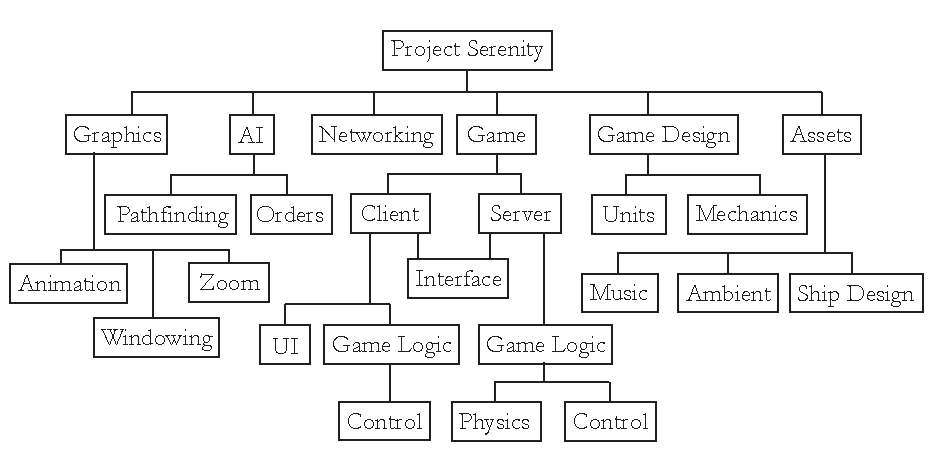
\includegraphics{res/wbs}
	\caption{Work Breakdown Structure of the game components}
\end{figure*}

From the WBS we can further break the project down into components which are suited for weekly development cycles.

Term 2 releases will include a UI, an AI system and further improvements to the components as required. Assets such as music and additional ship designs are non-essential and will likely follow in a later release.

\begin{figure}
	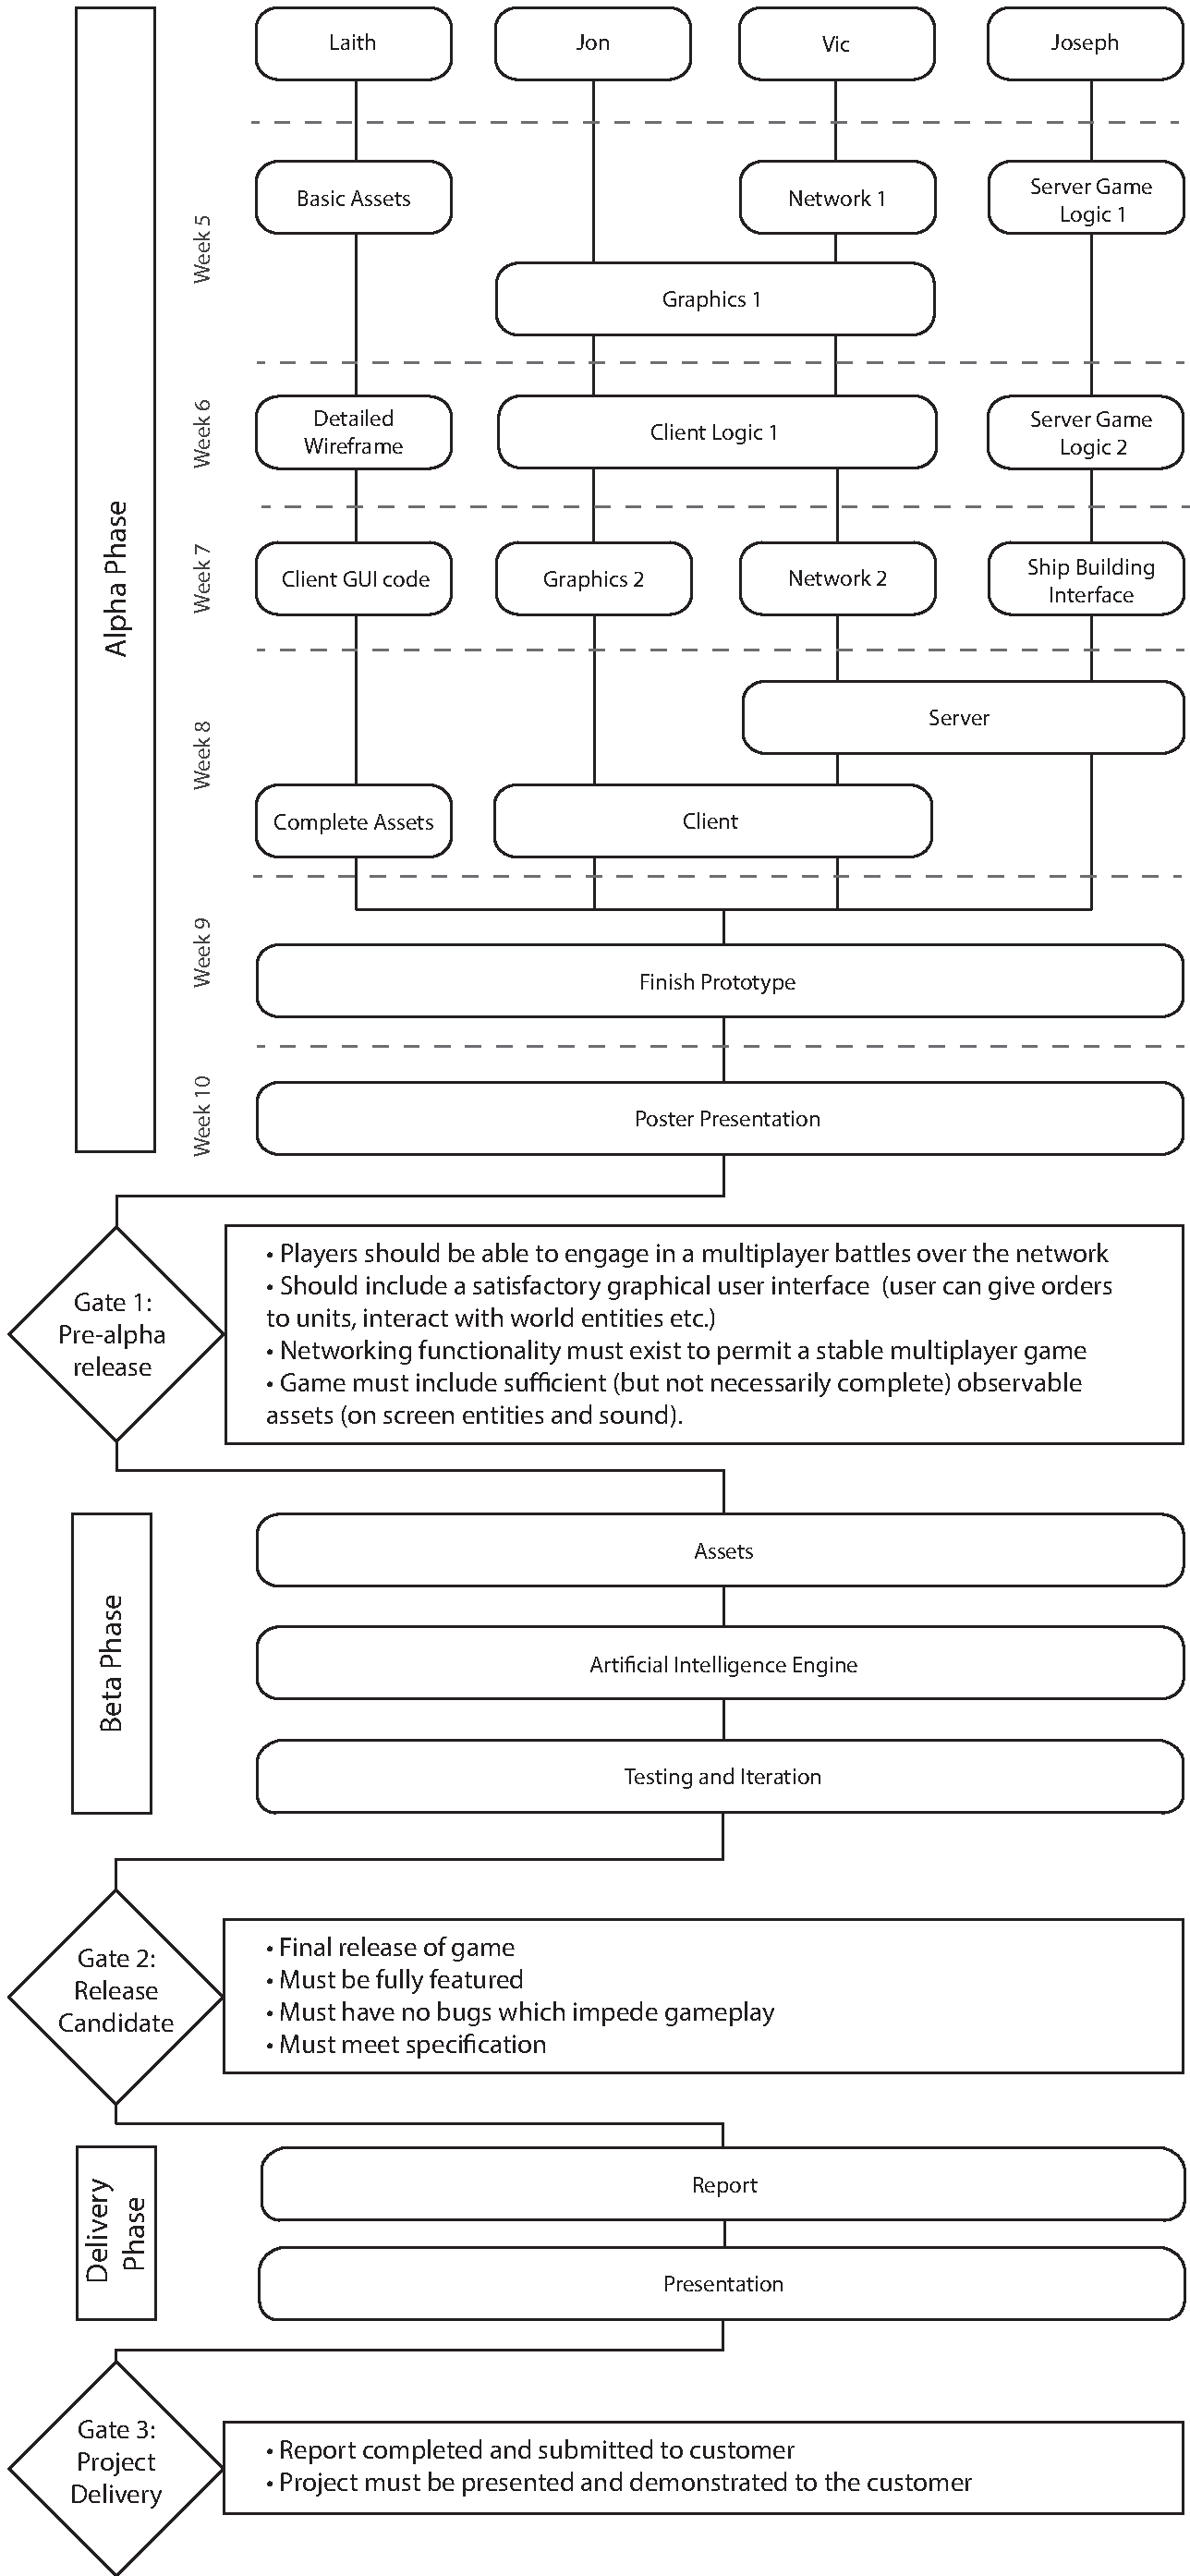
\includegraphics{res/stage_gate_diagram}
	% WE COULD PUT STANDARDS IN THE MARGIN!!! YES! CHEWING!!
	\caption{Stage-gate model of work breakdown structure showing the division of labour across the various project phases. 
	The alpha phase is more thoroughly planned so we are able to see a weekly breakdown of tasks in the near future. The gates are project milestones, each of which details the requirements for proceeding through that gate into the next phase.}
\end{figure}


	\section{Stakeholders and Communication Plan}
\label{section:communication}

The various parties identified as stakeholders are shown in Table \ref{tab:stakeholders} (overleaf). The relationship between the stakeholder and the project is shown, along with a rough estimate of their power and interest.\sidenote[][-2em]{See \bibentry{mendelow1991stakeholder}} This grid will form a reference for making sure that all interested parties are communicated with appropriately throughout the duration of the project.

\noindent Communication within the project team is examined in detail elsewhere in this document, so the remainder of this section is concerned with the other stakeholders.

\vspace{1em}

\begin{table*}
	\footnotesize
	\renewcommand{\arraystretch}{1.5}
	\begin{tabular}{p{9em} p{5em} p{3em} p{3em} p{9em} p{9em} p{9em}}
		\toprule
		\emph{Stakeholder} & \emph{Relationship} & \emph{Power} & \emph{Interest} & \emph{Requirements} & \emph{Measurements} & \emph{Communication Strategy} \\
		\midrule
		
		Project Team & Internal & High & High & 
		Good working environment, creative input. & 
		Meeting project spec, good grades! & 
		Various, detailed elsewhere. \\
		
		Supervisor --- Sara Kalvala & Internal & High & High & 
		Good communication. & 
		Adherence to spec, good PM, high quality write-up. & 
		Weekly meetings. \\
		
		Client --- Matt Leeke & Core \mbox{External} & High & High & 
		Good communication, creative input, hard work & 
		Strength of software, strength of report & 
		Weekly meetings. \\
		
		Second Assessor & Core \mbox{External} & High & Low & 
		None & 
		Marking scheme & 
		Deliverables only. \\
		
		Projects Organiser --- Steve Matthews & External & High & Low & 
		Cooperation when required. & 
		Deliverables on time. & 
		Email or meeting if required. \\
		
		Playtesters & External & Low & High & 
		Able to report issues / feature requests. & 
		Strength of game, input considered. & 
		Email. \\
		
		Other future users & Rest of World & Low & High & 
		Game works and is reliable. & 
		Strength of game, re-playability. & 
		Website, forums, blog. \\
		
		The Haskell and FP Communities & Rest of World & Low & High & 
		None & 
		Interest in  / strength of results and tools released. & 
		Online as above, and via the final report. \\
		\bottomrule
	\end{tabular}
	\vspace{1.5em}
	\caption[][1em]{Stakeholders for the project.}
	\label{tab:stakeholders}
\end{table*}

\subsection{Supervisor Meetings}

Regular communication with the project supervisor is likely to be a critical factor in success of the project. For this reason a weekly meeting with at least one member of the group if not more will be high priority.

\subsection{Client Meetings}

The client is clearly vital to the success of the project, and continual feedback on each release will allow for early identification of any problems. At least one meeting per release (ie each week) will be required, as well as further meetings and correspondence as needed.

\subsection{Projects Organiser and Second Assessor}

The projects organiser could exert a strong influence over the project if they wished, but as there are many projects and it would be inappropriate for them to demonstrate partiality, extended levels of communication are unlikely to be necessary. Brief updates pertaining to deliverables is all that should be required. But if the project organiser initiates communication then they should be made a high priority.

Communication with the second accessor is, for the most part, not appropriate, excepting when within the remit of the deliverables, i.e. the report and presentation themselves.

\subsection{Playtesters and End Users}

End users are clearly important to the goals of the project, but they will have little interest or influence in the early stages. Online updates, an email to report bugs to, and a mailing list for any events that are organised will be sufficient communication.

\subsection{The Haskell and Functional Programming Communities}

The overall end goal of the project is not just a game, but an examination of Haskell and Functional Programming as a game development environment. However the Haskell community at large is unlikely to have much interest in the project while it is running. Communication back to the community should therefore be largely via the final report, as well as the methods for end users above.



	\section{Quality Plan}
\label{section:quality}

\subsection{Playtesting}

\subsection{Unit Testing}

\subsection{Component Testing}

\subsection{Continuous Integration}

\subsection{Acceptance Testing}

\subsection{Stage Gate Model}
	\chapter[Job Descriptions]{Job Descriptions}
\label{ch:jobs}

\chapterepigraph{``Perhaps it hasn't one," Alice ventured to remark. ``Tut, tut, child!" said the Duchess. ``Everything's got a moral, if only you can find it."}{from Lewis Carol's  \emph{Alice in Wonderland}}

\newthought{Starting a sentence} with a new thought.

\section{A Section}

Lorum ipsum dolor sit amet.
    \section{Design Approach}

% how are we going about designing the game

% top down vs bottom up
% the advantages / disadvantages of both

Two methods were considered for our design approach: Top Down, and Bottom Up.
These are generic strategies for prioritising what to design first.

% Bottom Up
% used when existing off the shelf software is used
% integration between the existing software will take much longer
% licencing issues
% design sub parts of the game
Bottom Up typically starts with existing software modules that are integrated together to achieve a grander system.
Since the existing softwares provide the needed functionality, the majority of the implementation stage is piecing these software products/modules togother to form a cohesion product.
This approach falls short, when the software has to be written from scratch, since its focus is more on integration of existing products.

% Top Down
Top Down is used to design a system from scratch.
It's focus is on simplicity, only breaking down one aspect of the design at a time, into its smaller sub components.
The design Stage will continue to expand the subsystems of this design, until the subsystems begin to overlap with the implementation level, at this point, all further subsystem nodes are expanded at the implementation level.

% Conclusion
A hybrid approach will be used between the two design philosophies, at the design level, the  entire product will designed and implemented by the team, however at the implementation level, third party software products will be decided upon before the implementation stage, and will need factoring in to the design.

	\section{Risk Management}



Lorum ipsum sit dolor amet.\citefix{church1932}  \lipsum[2-4]
	\section{Legal, Ethical, and Social Issues}
\label{section:professional_issues}

% legal
One potential legal issue faced by this project is the use of third party software.
It must be ensured that any third party libraries included in the code are licensed
appropriately. This means only using software with a permissive license (e.g. Apache, BSD, or MIT licenses) and no proprietary software.

Game publishers such as Electronic Arts, and Lion Head, consider their games as intelligectual property, copywriting their games.
It is infeasable to check that all previous games published don't bear great similarities which would result in a court case.

% ethical


- gaming addiction
  - campaigns will be 5 battles long, allowing players an escape after 5 battles.

- dependency on whales (0.4\% of Zynga's customers account for 80\% of it's  1 billion profits.



% social issues
- language game in: english
- racism
- vialence




	\chapter[Forseeable Challenges]{Forseeable Challenges}
\label{ch:forseeable_challenges}

\chapterepigraph{The lurking suspicion that something could be simplified is the world's richest source of rewarding challenges}{Edsger Dijkstra}

\newthought{Some kind} of introductory paragraph.


\section{Time constraints}

Game development projects are famous for scheduling issues that threaten to delay the
release of a product. Developers often find themselves facing ``crunch time", a period
of extreme work overload, in an effort to deliver a game on time.\cite{groen2011}

This project only has approximately twenty weeks in which to develop a fully functioning
game that meets the requirements specified previously.

\section{Writing a successful AI}

Artificial intelligence can often be a make or break factor in determining the success of
a game.\citepage{rabin2002}{page 3} Without a convincing intelligence system, a game can
quickly become infuriating to play.

However, an AI system must be efficient as well as providing an entertaining experience.

\section{Minimal graphics libraries available}

Some investigation into the Haskell graphics libraries available has already been undertaken.
The Gloss package has been identified as a suitable candidate. Internally it
uses OpenGL, but exposes a clean functional API. Unfortunately it is a relatively simple
library and does not provide some required features such as windowing and clipping.

\section{Efficiency problems}

\part{Research\label{part:research}}
	\chapter[Current Trends in the Gaming Industry]{Current Trends in the Gaming Industry}
\label{ch:jobs}

\chapterepigraph{``Perhaps it hasn't one," Alice ventured to remark. ``Tut, tut, child!" said the Duchess. ``Everything's got a moral, if only you can find it."}{from Lewis Carol's  \emph{Alice in Wonderland}}

\newthought{Starting a sentence} with a new thought.

\section{A Section}

Lorum ipsum dolor sit amet.
	\chapter[Existing Games using Functional Programming Platforms]{Existing Games using Functional Programming Platforms}
\label{ch:existing_games}

\chapterepigraph{``Perhaps it hasn't one," Alice ventured to remark. ``Tut, tut, child!" said the Duchess. ``Everything's got a moral, if only you can find it."}{from Lewis Carol's  \emph{Alice in Wonderland}}

\newthought{Starting a sentence} with a new thought.

\section{A Section}

Lorum ipsum dolor sit amet.

	\chapter[IO, Networking, and Graphics --- Tackling the Awkward Squad]{IO, Networking, and Graphics --- Tackling the Awkward Squad}
\label{ch:awkward}

\chapterepigraph{``Perhaps it hasn't one," Alice ventured to remark. ``Tut, tut, child!" said the Duchess. ``Everything's got a moral, if only you can find it."}{from Lewis Carol's  \emph{Alice in Wonderland}}

\newthought{Starting a sentence} with a new thought.

\section{A Section}

Lorum ipsum dolor sit amet.

\part{Building the Game\label{part:main}}
	\section{Network Programming in Haskell}

Fast paced multiplayer games require efficient networking and real time packet delivery.
If this is not provided then the network can become a bottleneck causing the game to
lag or halt. This requirement means that the transmission control protocol (TCP) cannot
be used for game network development because of the implementation of reliability
in TCP. If a packet is lost when using TCP then the receiver stops and waits for that
data to be resent and any new data that is sent is held in a queue until the lost packet
arrives. Therefore, any packet loss on the network causes relatively large pauses in
communication which will cause objects in the game world to stop receiving updates and
the game hangs too.

So, networked multiplayer games that rely on real time network communications must use
the user datagram protocol (UDP) since it does not enforce a stop-and-wait style reliability system.
However, this means that a layer on top of UDP must also be used to implement an efficient
form of reliability, deal with duplicate packets and out of order packets, and create virtual
connections. Unfortunately, whilst Haskell provides a low level networking library, no suitable
library for game networking could be found, so one had to be developed. % XXX Reference chapter 3?

\subsection{Sending and Receiving Packets}

The \texttt{network} package is a low level networking interface that can be used to
send and receive packets using UDP.\sidenote{\url{http://hackage.haskell.org/package/network}}
It provides an easy to use API for creating and sending data over sockets.

\vspace{-0.5em}
\begin{listing}{list:recv}{Example of receiving UDP packets}{Example of receiving UDP packets}{}
\end{listing}\vspace{-1.5em}

\functions(main, port, withSocketsDo, socket, defaultProtocol, bind, socketPrint, recvFrom, putStrLn)
\begin{haskell}
>import Network.Socket
>
>port = 9900
>
>main :: IO ()
>main = withSocketsDo $ do
>  sock <- socket AF_INET Datagram defaultProtocol
>  bind sock (SockAddrInet port iNADDR_ANY)
>  socketPrint sock
>
>socketPrint :: Socket -> IO ()
>socketPrint sock = do
>  (msg, _, _) <- recvFrom sock 512
>  putStrLn msg
>  socketPrint sock

\end{haskell}
\noindent
Listing~\ref{list:recv} shows a simple UDP server which receives packets sent to port 9900
and prints the data that was received. First, this code initialises the networking subsystem
using "withSocketsDo". This is only necessary on machines running the Windows operating system,
but it is best practice to include this for portability. Then a UDP socket is created: "AF_INET"
indicates the use of IPv4, the "Datagram" socket type sets UDP, and a default protocol number
is set. The socket is bound to the specified listening port so that the operating system knows
to forward incoming packets on port 9900 to this socket. The socket is then passed to a loop
which reads incoming data with "recvFrom" and then prints it.

\vspace{-0.5em}
\begin{listing}{list:send}{Example of sending UDP packets}{Example of sending UDP packets}{}
\end{listing}\vspace{-1.5em}

\functions(main, port, withSocketsDo, socket, defaultProtocol, inet_addr, sendTo, close)
\begin{haskell}
>import Network.Socket
>
>port = 9900
>
>main :: IO ()
>main = withSocketsDo $ do
>  sock <- socket AF_INET Datagram defaultProtocol
>  addr <- inet_addr "127.0.0.1"
>  sendTo sock "Hello world!" (SockAddrInet port addr)
>  close sock

\end{haskell}
\noindent
Sending a packet, as shown in Listing~\ref{list:send}, is just as simple. This is a very basic
UDP client that creates a socket and sends a string to port 9900 on the local machine. "inet_addr"
is used to convert a "String" into a network address in host byte order. This address can
then be used as part of an argument that specifies the destination for the "sendTo" function.
Finally the program cleans up after itself by closing the socket.

These two examples show how simple it is to develop basic networking functionality in Haskell.
However, UDP alone, as mentioned previously, is not robust enough to be used for games on real
world networks which experience packet loss and packets arriving out of sequence. So, the next
step is to develop a virtual connection over UDP.

\subsection{Connections over UDP}


\subsection{Reliability}


\subsection{Networking threads}

% Inbox + outbox loops
% TChans
% ConnectionMap
	
	\section{Choosing a Graphics Framework}

% OpenGL, Gloss etc

\begin{marginfigure}
	\includegraphics{res/gloss/gloss-tree.png}
	\vspace{1em}
	\includegraphics{res/gloss/gloss-styrene.png}
	\caption[Gloss example screens.]{Gloss example screens from \url{gloss.ouroborus.net/}.}
	\label{fig:gloss}
\end{marginfigure}

Any game is clearly going to involve graphics in some capacity or another, but graphics are not something that at first sight seem suited to a functional language. There are, however, various graphical frameworks and bindings available for Haskell.

For the purposes of the Serenity project, the choice basically boiled down to three options. Firstly, there are bindings directly to OpenGl available; which would provide the most flexibility but also likely the most development time. Secondly there are the bindings to the SDL engine, along with all the various tools provided with its framework. Many of the existing games written in Haskell use SDL. Lastly there is the use of the simple but effective layer over GLUT and OpenGL provided by the Gloss library.

This was not an easy decision, and some time went into making it. The direction taken in the Serenity project was to use the Gloss library, mostly because of its simple interface and ease of use, given the limited time and large scope of the rest of the project. The advantages of Gloss can be appreciated by considering the two screens in Figure \ref{fig:gloss}. Both of these examples involve relatively simple code, which is almost entirely pure.

The decision to use Gloss has largely been held up, but there has been some problems due to features it lacks, the most notable being clipping. In the future it would probably be beneficial to replace Gloss with an in house framework providing a layer between the pure graphics code and impure bindings to OpenGL. (This is discussed further in the next section.)

\paragraph{Summary of this section} Given the limited time available for the Serenity project, the prebuilt pure interface onto OpenGL provided by the Gloss library was the best option, and this has been born out by the results. A custom made layer that is more appropriate for the needs of a complex game, and more readily adapted to changing requirements, would be beneficial to develop in the future.

	\input{chapter/main/ai}
	\section{Testing}
\label{section:testing}

% How we used the different test frameworks

Lorum ipsum sit dolor amet.\citefix{church1932}  \lipsum[2-4]

	\input{chapter/main/manual}
\part{Project Evaluation\label{part:evaluation}}
	\input{chapter/evaluation/game}	
	\input{chapter/evaluation/haskell}
	\chapter[Project Management]{Project Management}
\label{ch:management}

\chapterepigraph{``All things are created twice; first mentally; then physically.  The key to creativity is to begin with the end in mind, with a vision and a blue print of the desired result."}{ Stephen Covey}

\newthought{Starting a sentence} with a new thought.

Our project team has adopted the agile development cycle as a basis for our management structure. We've broken the project down into critical components and have committed to weekly releases to ensure the project remains well scheduled throughout the project lifetime.

\section{Risk Management}



Lorum ipsum sit dolor amet.\citefix{church1932}  \lipsum[2-4]
\section{Grievance Policy}
It's imperative to document a grievance guideline to ensure that any grievance procedures are fair and impartial. %ref gov
 Because the developer team is small, an internal dispute would have a high cost to the project, so grievance issues need to be dealt with promptly. 
  
\begin{enumerate}[i)]
    \item{Attempt to resolve the grievance issue informally by the team manager.}
    \item{If the issue cannot be resolved informally, and affects the entire project group, then address the issue at the next meeting and attempt to find a resolution in a group environment.}
    \item{If the issue cannot be solved by a formal group meeting then a managerial confrontation is required to reduce the impact on the project.}
    \item{If the issue still cannot be resolved then a complaint should be made to the module supervisor and university procedure should be followed from then on.}
\end{enumerate}

\section{Weekly Releases}
As a motivating factor to keep the project on schedule we've committed to component releases every Tuesday evening. The release should include the latest completed iteration of the project, which is scheduled to develop as a prototype by the end of term 1.

\section{Standup Meetings}
Standup meetings are held every week to discuss individual progress on the project, any issues an individual has been encountered, and what they will attempt to accomplish in the following week.

\section{Change Management}
\begin{figure*}[h!]
\includegraphics{"res/Change management diagram"}
\caption{Change management workflow}
\end{figure*}
\section{Tools and Techniques}

\section{Develop}

Whatever that means...
\part{Into the Future\label{part:future}}
	\input{chapter/future/library}
	\input{chapter/future/game}

\part{Appendices and Indices\label{part:appendices}}

\backmatter

\chapter{Acknowledgements}

\begin{fullwidth}

\lipsum[1]

\vspace{1em}\noindent
This report makes extensive use of the Tufte Latex class written by Bil Kleb, Bill Wood, and Kevin Godby (\url{http://code.google.com/p/tufte-latex/}). 
The Haskell code in this report was typeset using a modified version of Lambda\TeX\ originally created by Patryk Zadarnowski (\url{http://www.jantar.org/lambdatex/}).

\end{fullwidth}

\begin{fullwidth}

\def\bibname{Full Reference List and Selected Bibliography}
\nocite{*}
\bibliographystyle{plainnat}
\addcontentsline{toc}{chapter}{\bibname}
\bibliography{references}

\cleardoublepage
\phantomsection \label{listoflis}
\addcontentsline{toc}{chapter}{List of Listings}
\listofvlisting

\cleardoublepage
\phantomsection \label{listoffig}
\addcontentsline{toc}{chapter}{List of Figures}
\listoffigures

\end{fullwidth}
\printindex

\end{document}
